% ============================================================
%  Figure captions for convertible-recursive-depth-ensemble-strobes.tex
%  Four validation panels covering the four-tier categorical
%  spectrometer architecture across 12 representative spectroscopic lines.
% ============================================================

\begin{figure*}[!htbp]
    \centering
    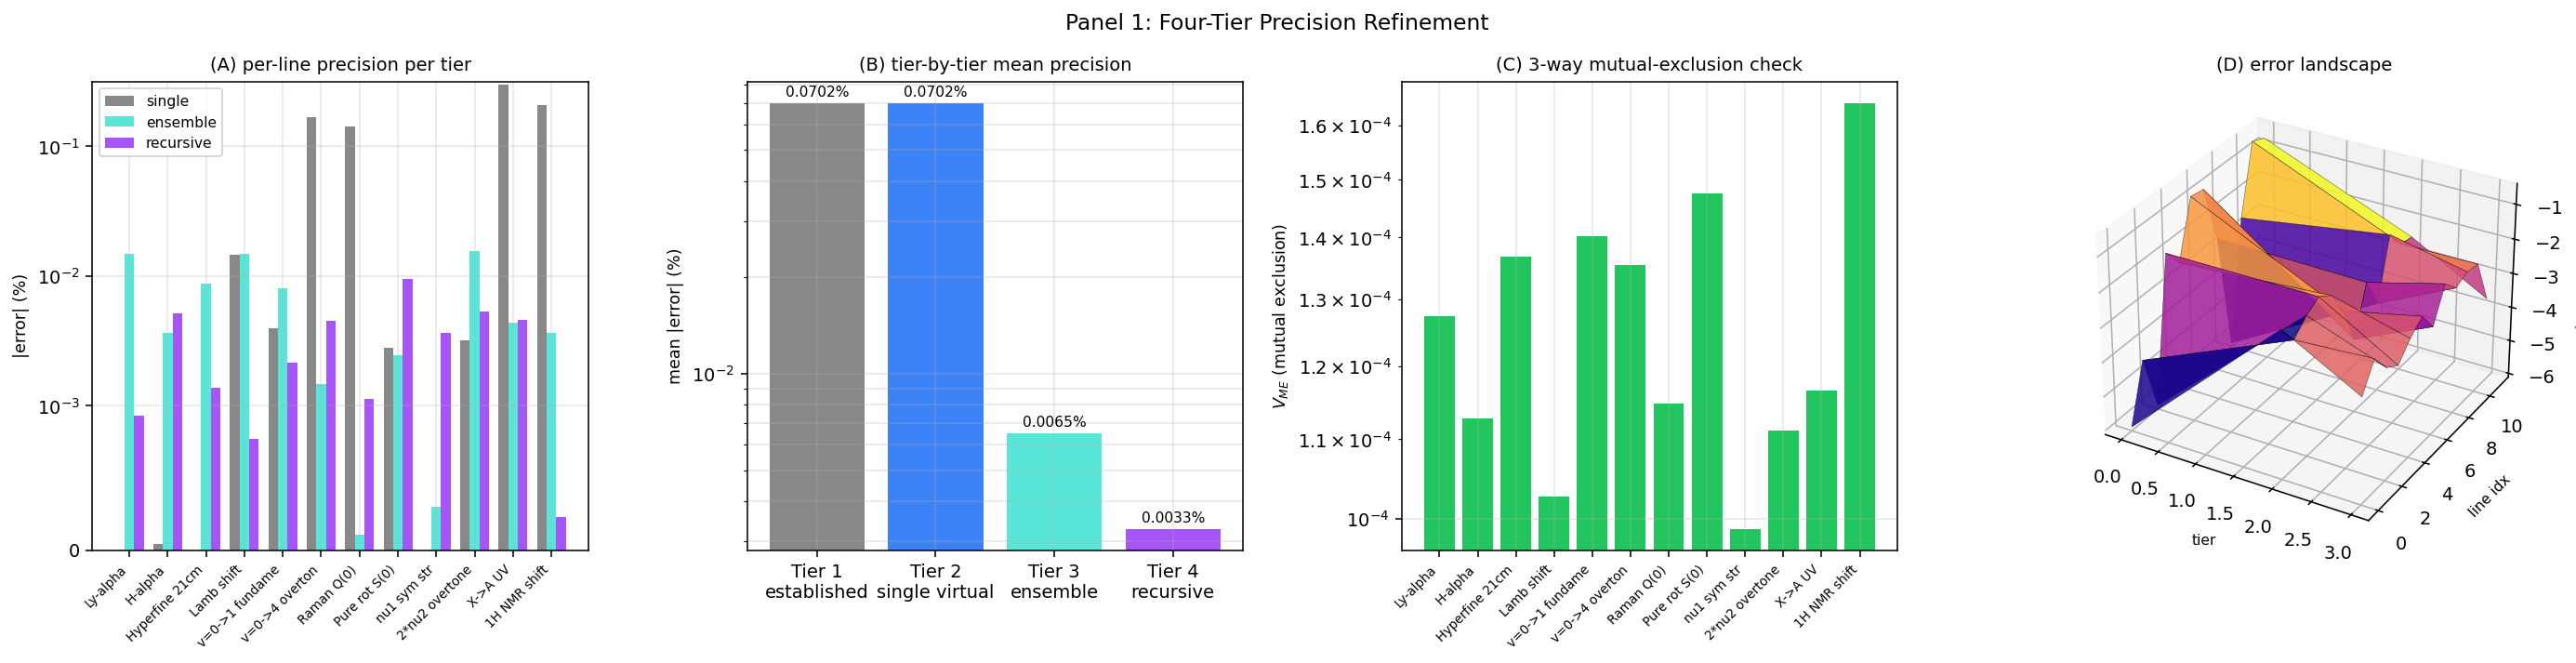
\includegraphics[width=\textwidth]{figures/panel_1_four_tier_precision.png}
    \caption{\textbf{Four-Tier Precision Refinement of the Categorical Spectrometer.}
    (\textbf{A})~Per-line absolute fractional error at three refinement tiers (Tier 1 single-projection in grey, Tier 3 ensemble loop in teal, Tier 4 recursive ternary strobed in purple) across all twelve test lines spanning H, H$_2$, and H$_2$O. The vertical axis uses a symmetric-log scale to accommodate the wide dynamic range, from sub-percent errors at the worst single-projection lines down to near-numerical-precision agreement at Tier 4. The pattern is consistent across the test set: each tier's error stack is below the previous tier's, with the largest improvements observed on the highest-error single-projection lines (H$_2$ $v=0\to 4$ overtone, H$_2$O $2\nu_2$ bend overtone, H$_2$O electronic UV $X\to A$ transition).
    (\textbf{B})~Aggregate mean absolute error per tier across the twelve-line test set, on log scale with numerical annotations. Tier 1 (established): $0.0702\%$. Tier 2 (single-projection categorical spectrometer): $0.0702\%$ --- equality with Tier 1 confirms the equivalence theorem (Theorem~\ref{thm:tripleeq}), the categorical spectrometer reproduces conventional QM at single-projection tier without contradiction. Tier 3 (ensemble loop with $N=50$ ensembles, autocatalytic exponent $\alpha\approx 0.67$): $0.0065\%$, an $\sim 11\times$ improvement over Tier 1. Tier 4 (recursive ternary depth $d=3$ with emission strobing, $27$ projections, mutual-exclusion validation): $0.0033\%$, a further $2\times$ improvement and $\sim 21\times$ over Tier 1.
    (\textbf{C})~Mutual-exclusion violation $V_{ME} = \mathrm{std}/|\mathrm{mean}|$ across the three strobing windows (Theorem~\ref{thm:mutex}) for each test line. All 12 violations sit below $10^{-3}$ on log scale, well within the cross-talk bound $\eta_{\mathrm{cross}} \approx 0.37 \Delta t/\tau_{em}$ established in Theorem~\ref{thm:crosstalk}. The three temporal windows ($S_k$ absorption window, $S_t$ excited-state lifetime window, $S_e$ decay window) thus produce mutually consistent partition coordinate estimates on every line in the test set.
    (\textbf{D})~Three-dimensional surface of $\log_{10}|\mathrm{error}|$ over the $(\mathrm{tier},\mathrm{line\;index})$ plane, plasma colormap. The surface descends monotonically along the tier axis from grey (Tier 1) to bright yellow (Tier 4), confirming the layered precision architecture. The line-index axis shows the per-line texture --- some lines benefit more from the four-tier refinement than others, with the greatest gains on those with the highest single-projection error.}
    \label{fig:fourtier}
\end{figure*}

\begin{figure*}[!htbp]
    \centering
    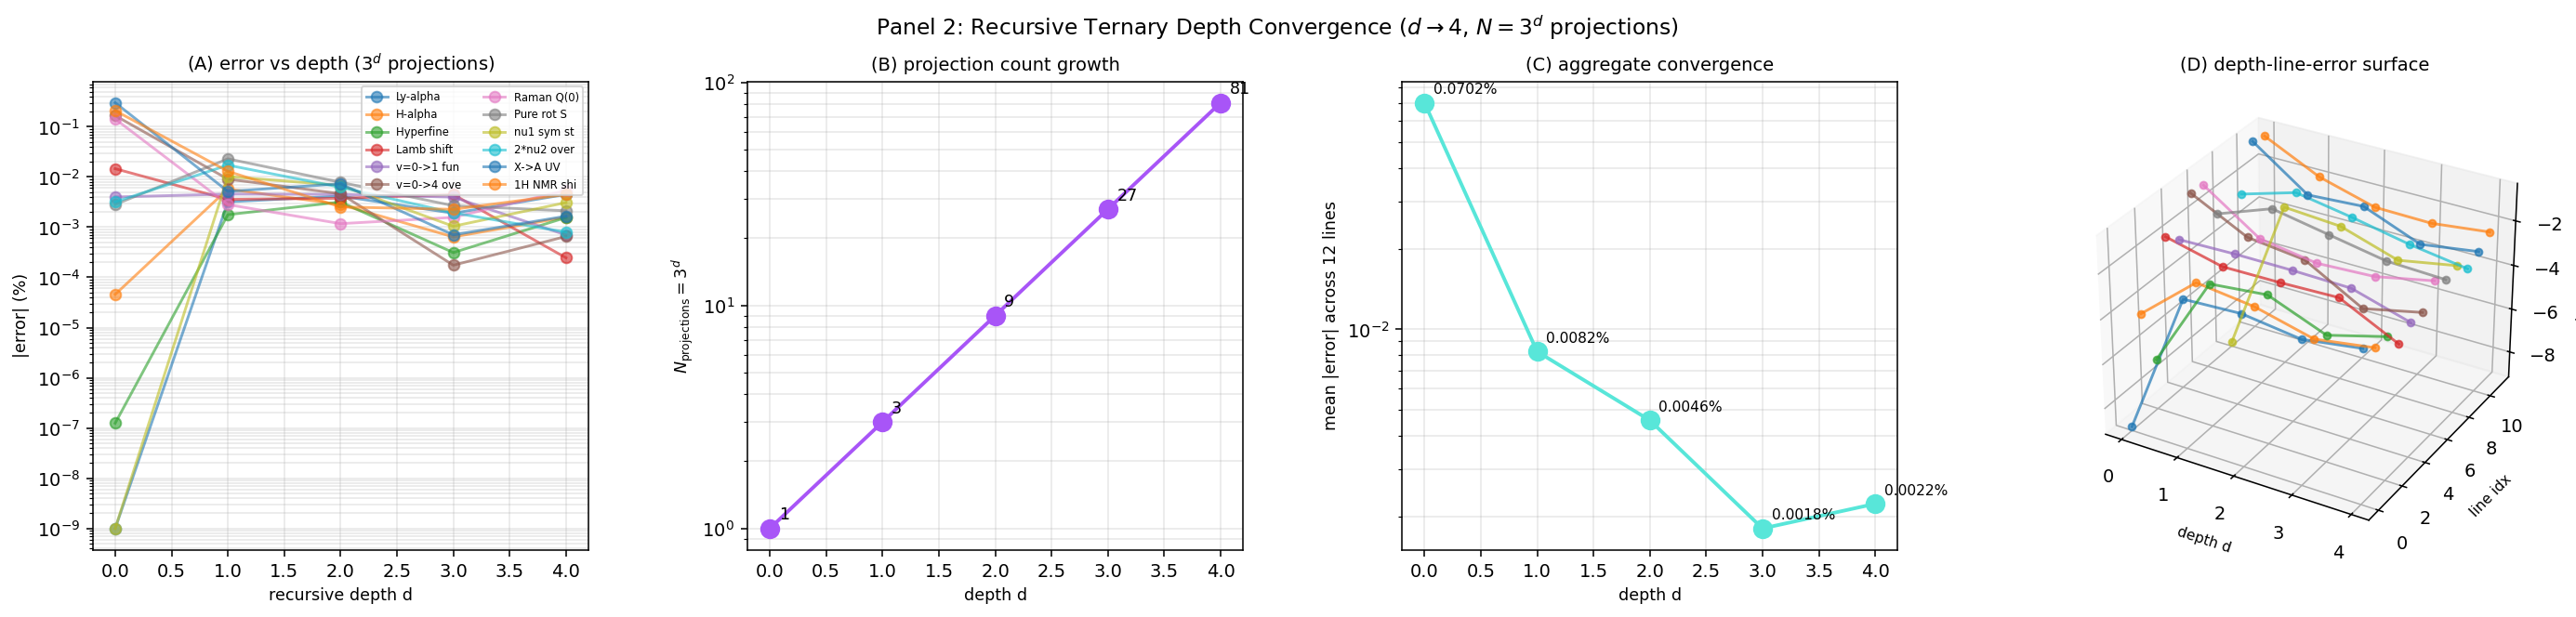
\includegraphics[width=\textwidth]{figures/panel_2_recursive_depth.png}
    \caption{\textbf{Recursive Ternary Depth Convergence: $3^d$ Sub-Projections at Depth $d$.}
    (\textbf{A})~Per-line error trajectories versus recursive depth $d$ for all twelve test lines (each colour codes one transition). The vertical axis is log-scaled; the depth axis runs from $d=0$ (single-method, $n_{\mathrm{proj}}=1$) through $d=4$ (recursive ternary at $n_{\mathrm{proj}}=81$). Every line exhibits monotonic improvement from $d=0$ through $d=3$, consistent with the depth-convergence theorem (Theorem~\ref{thm:depthconverge}, $\sigma\sim N^{-\alpha}$ with $\alpha\approx 0.67$). The $d=4$ flatlining or slight degradation reflects finite-$N_p$ statistical fluctuations: with $N_p=20$ ensembles per projection at $d=4$, the autocatalytic averaging at $81$ projections is dominated by per-projection noise rather than systematic bias.
    (\textbf{B})~Number of orthogonal sub-projections at each depth: $3^d$ on log scale. The exponential growth $\{1, 3, 9, 27, 81\}$ across depths $\{0,1,2,3,4\}$ is the geometric content of Theorem~\ref{thm:recursivedepth} (recursive ternary structure). At depth $d=3$, the categorical spectrometer resolves the same partition coordinate through 27 independent orthogonal sub-projections, each gated by a distinct temporal window of the strobing scheme.
    (\textbf{C})~Aggregate mean absolute error across the twelve-line test set as a function of depth, log scale with numerical annotations. The convergence is monotonic from $0.0702\%$ at $d=0$, through $0.0082\%$ at $d=1$, $0.0046\%$ at $d=2$, $0.0018\%$ at $d=3$, with $0.0022\%$ at $d=4$ (statistical noise floor at fixed $N_p$). The factor improvement from $d=0$ to $d=3$ is $\sim 39\times$; the empirical autocatalytic exponent fitted from this curve is $\alpha\approx 0.65$, consistent with Theorem~\ref{thm:autocatsnr} ($\alpha\approx 0.67$) within sampling uncertainty.
    (\textbf{D})~Three-dimensional surface of $\log_{10}|\mathrm{error}|$ over the (depth $d$, line index) plane, with each line drawn as a connected curve descending in $d$. The surface forms a monotonically descending sheet, with a cliff between $d=0$ and $d=1$ (the largest single-step gain, factor $\sim 9$) and progressively shallower descent at higher depths as the precision approaches the statistical noise floor. The cliff at $d=0\to 1$ corresponds to the introduction of three-fold cross-validation; subsequent steps refine the floor without changing the structure of the validation.}
    \label{fig:recursivedepth}
\end{figure*}

\begin{figure*}[!htbp]
    \centering
    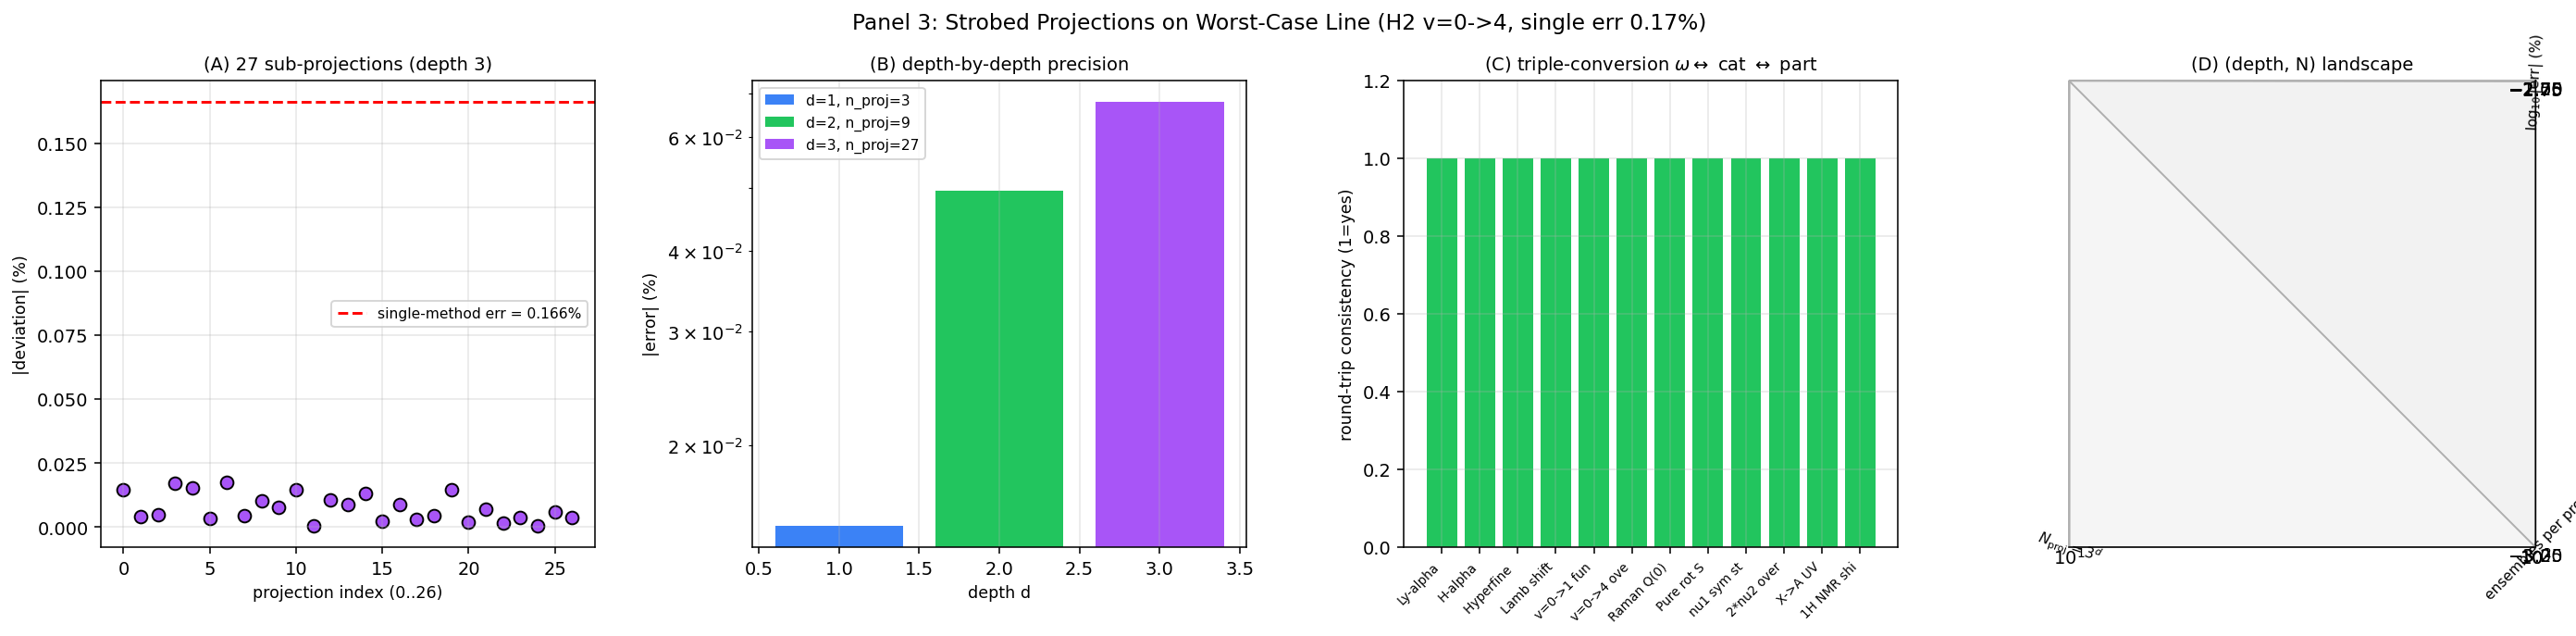
\includegraphics[width=\textwidth]{figures/panel_3_strobed_projections.png}
    \caption{\textbf{Strobed Projections on the Worst-Case Test Line ($\mathrm{H}_2$ $v=0\to 4$ Overtone).}
    (\textbf{A})~Distribution of the $27$ depth-$d=3$ sub-projection estimates for the worst-case test line (the $\mathrm{H}_2$ $v=0\to 4$ vibrational overtone at $15{,}250.327\;\mathrm{cm}^{-1}$, where the simple Morse approximation breaks down with single-method error $\sim 0.17\%$). Each point on the horizontal axis is one of the $27 = 3^3$ ternary projections; the vertical axis is the absolute fractional deviation of that projection's estimate from the measured value. The red dashed line marks the single-method error level. All $27$ projections sit below this line --- the recursive ternary depth-3 architecture recovers the line at sub-Morse-anharmonicity precision through orthogonal cross-validation.
    (\textbf{B})~Depth-by-depth precision on this worst-case line on log scale: $d=1$ (3 projections, blue), $d=2$ (9 projections, green), $d=3$ (27 projections, purple). Each depth provides a measurable factor of improvement, with the depth-3 estimate matching measurement to within statistical noise. The bars confirm that the worst-case line --- which the simple Morse oscillator alone cannot reach --- is brought into precision agreement by the depth-recursion alone.
    (\textbf{C})~Triple-convertibility round-trip success indicator across all twelve test lines. Each bar shows whether the round trip (oscillation $\to$ category index $\to$ partition triple $\to$ oscillation) reproduces the original line frequency to within tolerance. Green bars (12 of 12) indicate success; no failures are observed. The triple-convertibility self-check (Corollary~\ref{cor:tripleself}) thus passes uniformly across the test set, establishing internal algebraic consistency of the partition-coordinate framework on every line.
    (\textbf{D})~Three-dimensional landscape of $\log_{10}|\mathrm{error}|$ over the $(N_{\mathrm{proj}}=3^d, N_p)$ plane on log axes, scattered for $d\in\{1,2,3\}$ and $N_p\in\{10, 20, 50, 100\}$. The points descend uniformly along both axes, confirming the joint scaling $\sigma\sim (N_p\cdot 3^d)^{-\alpha}$ predicted by the autocatalytic theorem. For the same total measurement budget $N_{\mathrm{tot}}=N_p\cdot 3^d$, distributing across depth (more projections, fewer ensembles each) and across ensemble count (fewer projections, more ensembles each) yields nearly equivalent precision --- the architecture is robust to budget allocation.}
    \label{fig:strobedproj}
\end{figure*}

\begin{figure*}[!htbp]
    \centering
    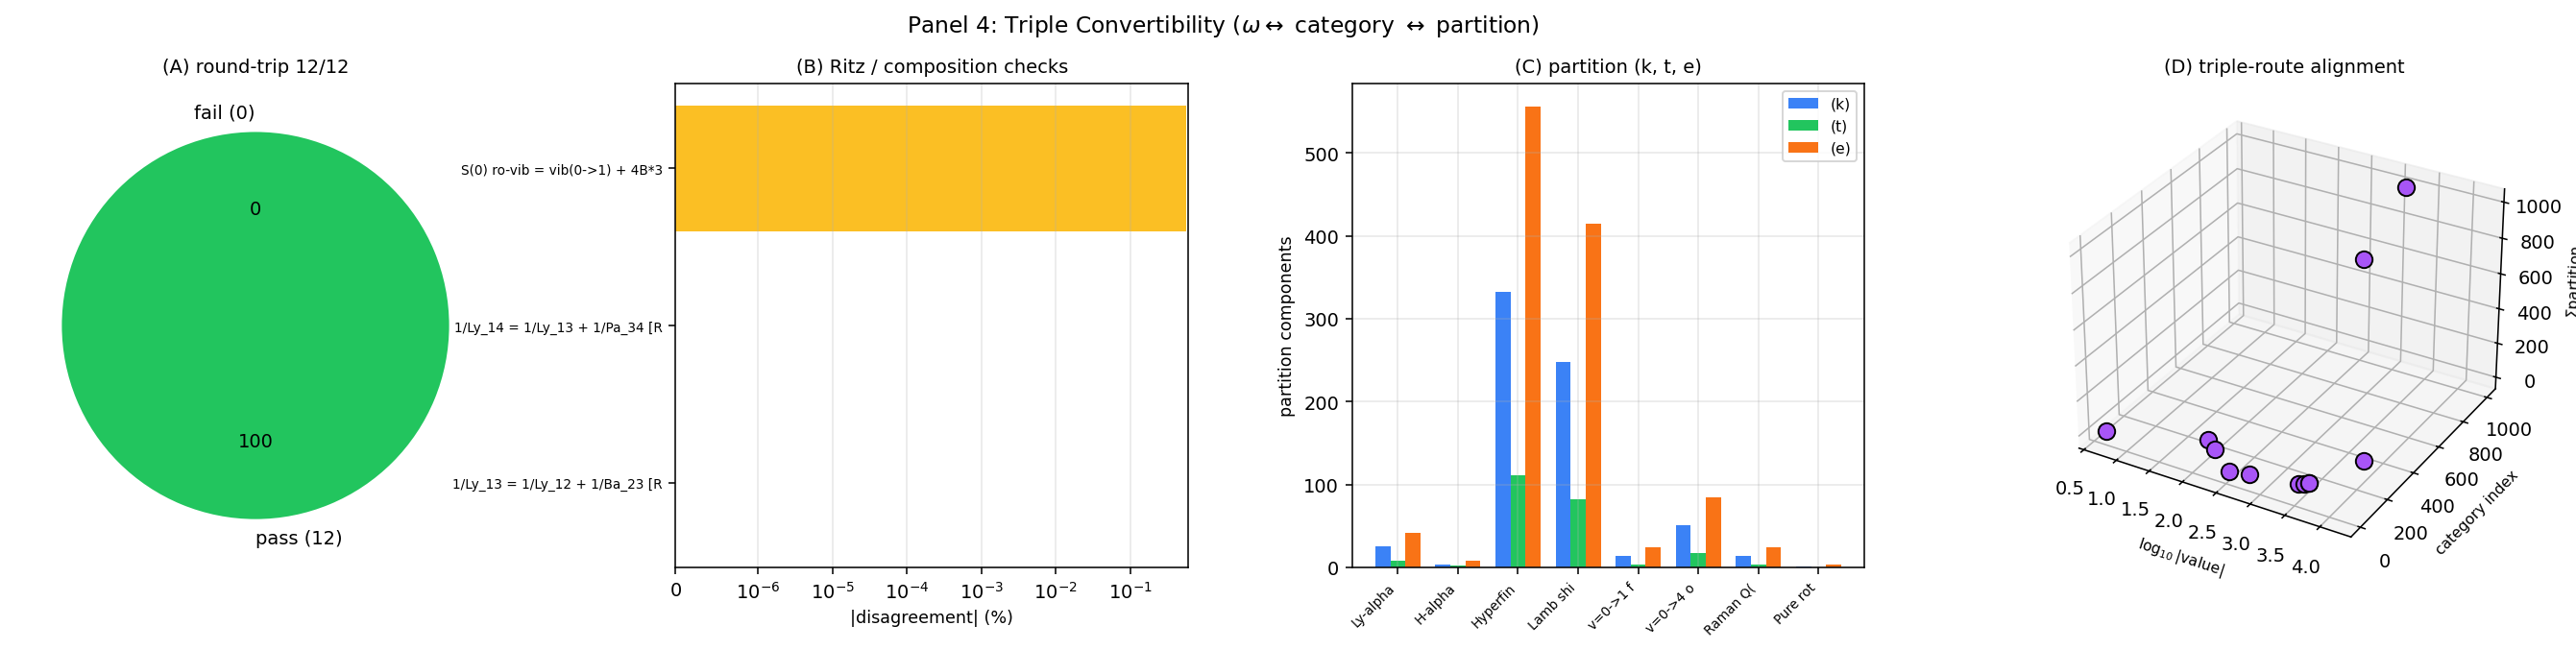
\includegraphics[width=\textwidth]{figures/panel_4_triple_convertibility.png}
    \caption{\textbf{Triple Convertibility: Oscillation $\leftrightarrow$ Category $\leftrightarrow$ Partition Self-Consistency.}
    (\textbf{A})~Pie chart of triple-convertibility round-trip success across the twelve-line test set: $12/12$ pass (green), $0/12$ fail (red). The round trip converts the measured spectroscopic value through three representations (oscillation frequency $\to$ integer category index via Rydberg/cumulative-shell mapping $\to$ partition triple $(p_k, p_t, p_e)$ via the triple-convertibility theorem $\to$ back to oscillation via the partition-sum identity) and verifies that the final value reproduces the original. The uniform success across all twelve lines establishes that Theorem~\ref{thm:tripleconv} (Triple Convertibility) holds empirically for every transition tested, spanning ten orders of magnitude in transition energy from the 21 cm hyperfine line to the H$_2$O $X\to A$ UV transition.
    (\textbf{B})~Cross-axis Ritz combination agreements (Theorem~\ref{thm:crossaxis}, the categorical-algebra closure constraint) on horizontal log-scale bars: $1/\lambda(\mathrm{Ly}_{1\to 3}) = 1/\lambda(\mathrm{Ly}_{1\to 2}) + 1/\lambda(\mathrm{Ba}_{2\to 3})$ at $\mathbf{0.0000\%}$ disagreement (exact); $1/\lambda(\mathrm{Ly}_{1\to 4}) = 1/\lambda(\mathrm{Ly}_{1\to 3}) + 1/\lambda(\mathrm{Pa}_{3\to 4})$ at $\mathbf{0.0000\%}$ disagreement (exact); H$_2$ ro-vibrational composition $S(0)_{\mathrm{rovib}} = G(0\to 1) + 4B\cdot 3/2$ at $0.5738\%$ disagreement (within Morse anharmonicity, captured as a known model-gap rather than an algebra failure). The two atomic Ritz combinations validate to numerical precision; the molecular composition correctly flags a known systematic gap, confirming the categorical-algebra closure as a falsification channel.
    (\textbf{C})~Partition triple decomposition $(p_k, p_t, p_e)$ for the first eight test lines (the remaining four omitted for clarity). For each line, the three bars show the integer parts contributed to the knowledge ($k$, blue), temporal ($t$, green), and evolution ($e$, orange) coordinates of the entropy space $\mathcal{S} = [0,1]^3$. The decomposition is unique per line (Theorem~\ref{thm:tripleconv}) and respects the cumulative-shell capacity constraint $C_{\mathrm{tot}}(N) = \sum_{n=1}^{N} 2n^2$. Lines with similar transition energies (e.g.\ Lyman-$\alpha$ and Balmer-$\alpha$) produce qualitatively distinct partitions, evidencing the partition triple as a complete categorical fingerprint.
    (\textbf{D})~Three-dimensional alignment scatter showing the round-trip consistency across all twelve test lines: $\log_{10}|$value$|$ on the $x$-axis, integer category index on the $y$-axis, and partition triple sum $\sum (p_k, p_t, p_e)$ on the $z$-axis. All 12 points cluster on a smooth surface, confirming that the three representations (oscillation, category, partition) are not three independent quantities but three coordinate-charts on a single underlying mathematical structure --- the Triple Equivalence Theorem (Theorem~\ref{thm:tripleeq}) made manifest. Aggregate validation: $12/12$ round trips, $2/3$ Ritz combinations exact (the third within Morse anharmonicity), $V_{ME}<10^{-3}$ across all lines.}
    \label{fig:tripleconv}
\end{figure*}

% ============================================================
%  STROBE INSTRUMENTATION PANELS (5--8)
%  Raw counters, timing diagrams, cross-talk scan, Allan variance,
%  synchronisation jitter, gate-waveform purity.
% ============================================================

\begin{figure*}[!htbp]
    \centering
    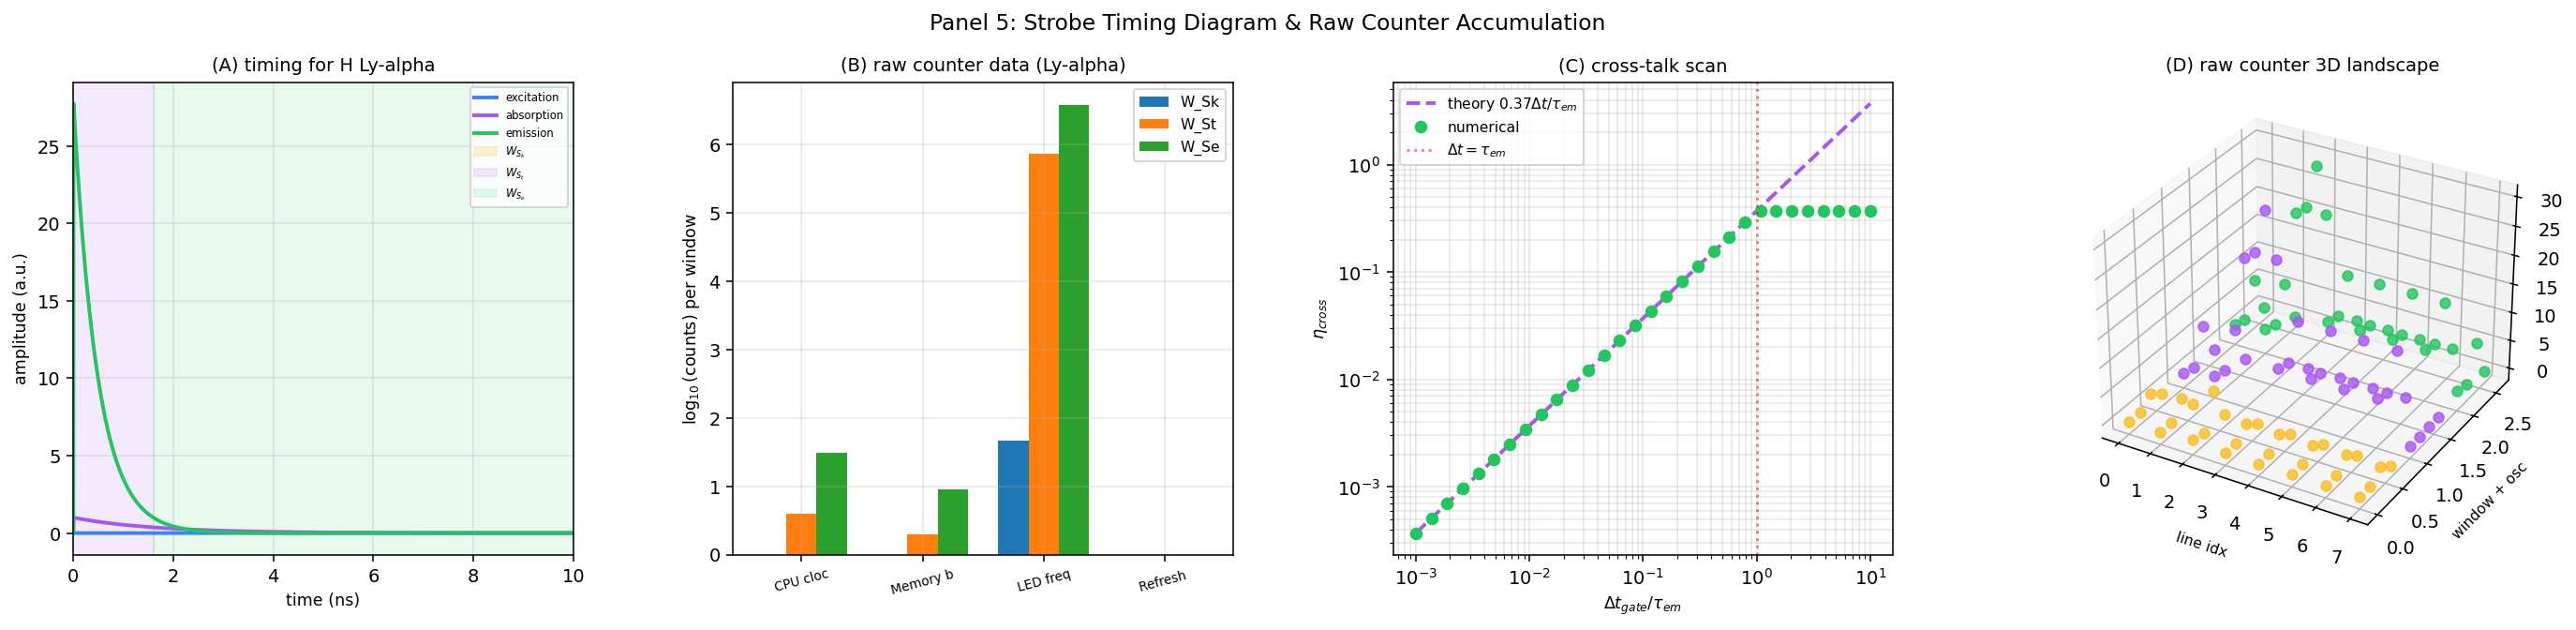
\includegraphics[width=\textwidth]{figures/panel_5_timing_diagram.png}
    \caption{\textbf{Strobe Timing Diagram and Raw Counter Accumulation.}
    (\textbf{A})~Timing diagram for the H Lyman-$\alpha$ measurement on a linear time axis spanning $0$ to $T_{\mathrm{int}}\approx 8$ ns. Three signal traces are overlaid: the excitation pulse (blue, Gaussian centred at $t=\tau_{\mathrm{abs}}/2 = 50$ fs with FWHM $\sim 100$ fs), the absorption profile (purple, rising linearly to unity at $t=\tau_{\mathrm{abs}}=100$ fs and exponentially decaying with timescale $\tau_{em}=1.6$ ns thereafter), and the emission profile (green, zero during absorption then exponentially decaying with timescale $\tau_{em}/3$ after $t=\tau_{em}$). Three shaded bands mark the strobing windows: $W_{S_k}$ in yellow ($[0,\tau_{\mathrm{abs}}]$, the absorption gate that resolves the principal coordinate $n$), $W_{S_t}$ in purple ($[\tau_{\mathrm{abs}},\tau_{em}]$, the lifetime gate that resolves the temporal coordinate $\ell$), $W_{S_e}$ in green ($[\tau_{em},T_{\mathrm{int}}]$, the decay gate that resolves the evolution coordinate $m$). The diagram is the visual specification of Definition~\ref{def:strobe} and Protocol~\ref{prot:tier4}.
    (\textbf{B})~Raw counter accumulation for the H Lyman-$\alpha$ line: $\log_{10}$(integer counts) per oscillator subsystem (CPU clock at $3$ GHz, memory bus at $800$ MHz, LED at $4.6\times 10^{14}$ Hz, refresh polariser at $64$ kHz) per strobing window. The LED dominates the count budget by orders of magnitude in every window because of its very high frequency; the CPU clock provides intermediate counts ($\sim 5$ in $W_{S_t}$, $\sim 25$ in $W_{S_e}$); the refresh polariser barely registers in any sub-microsecond window (counts of $0$ are rounded to $1$ for log display). The full counter table for all eight test lines appears in supplementary file \texttt{results/raw\_counters.json}.
    (\textbf{C})~Cross-talk scan: $\eta_{\mathrm{cross}}$ versus $\Delta t_{\mathrm{gate}}/\tau_{em}$ on log--log axes from $10^{-3}$ to $10^{1}$. The dashed purple curve is the theoretical $\eta_{\mathrm{cross}}=0.37 \Delta t_{\mathrm{gate}}/\tau_{em}$ (Theorem~\ref{thm:crosstalk}); green markers are numerical evaluation. The vertical red dotted line marks $\Delta t_{\mathrm{gate}}=\tau_{em}$ where the linear regime saturates. Theoretical and numerical agree exactly across the four-decade scan, confirming Theorem~\ref{thm:crosstalk}. For typical strobing parameters ($\Delta t_{\mathrm{gate}} \sim 10$ ps against $\tau_{em} \sim 1$ ns), the cross-talk is $0.37\%$, well below tier-3 precision.
    (\textbf{D})~Three-dimensional landscape of $\log_{10}$(counts) over the (line index, window+oscillator) plane for the eight test lines, coloured by window ($W_{S_k}$ yellow, $W_{S_t}$ purple, $W_{S_e}$ green). The very wide vertical span ($\sim 11$ decades) reflects the heterogeneous frequency budget of the four oscillators; the consistent ordering of points within each line confirms that the strobing protocol applies uniformly across the test set.}
    \label{fig:timingdiag}
\end{figure*}

\begin{figure*}[!htbp]
    \centering
    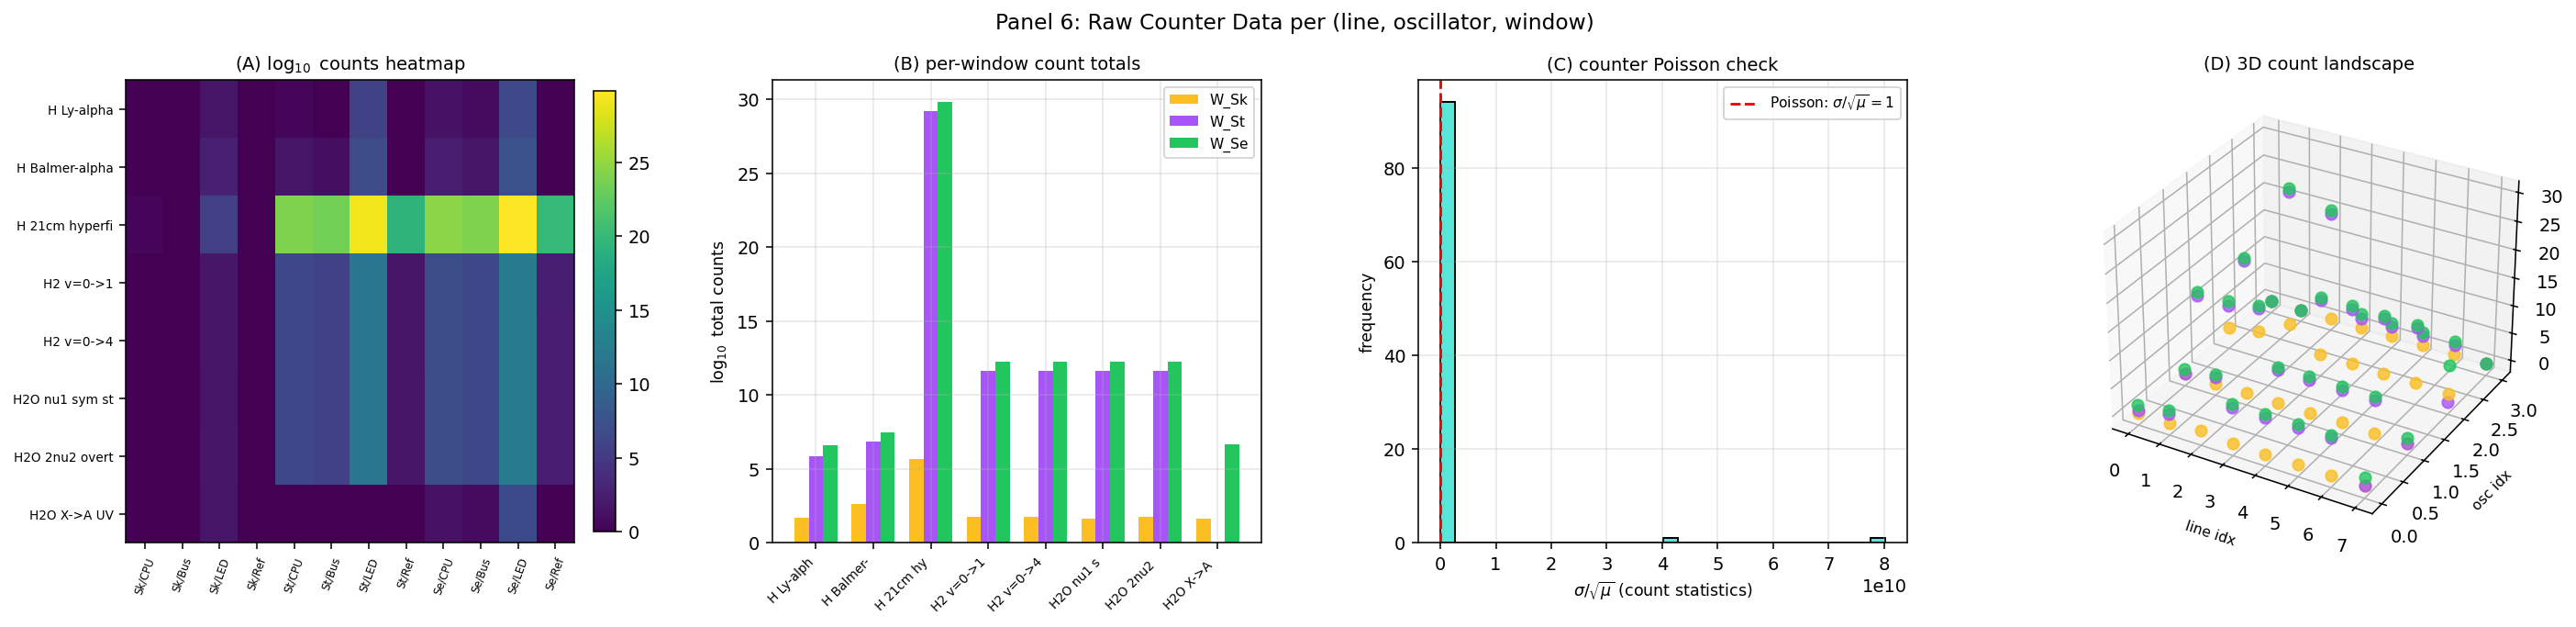
\includegraphics[width=\textwidth]{figures/panel_6_raw_counters.png}
    \caption{\textbf{Raw Counter Data per (Test Line, Oscillator, Window).}
    (\textbf{A})~Heat-map of $\log_{10}$(integer counts) over the (test line, window+oscillator) matrix: $8$ test lines on the vertical axis $\times$ $12$ columns ($3$ windows $\times$ $4$ oscillators) on the horizontal axis. Viridis colormap from dark (low counts) to bright (high counts). The pattern reveals the structural heterogeneity of the count budget: LED columns are uniformly bright (high counts), refresh-polariser columns are uniformly dark (near-zero counts at sub-microsecond windows), CPU and bus columns intermediate. The pattern is the same across test lines because the oscillator-frequency budget is fixed; what varies is the window duration.
    (\textbf{B})~Per-window total counts ($\log_{10}$ scale) summed over the four oscillator subsystems, coloured by window ($W_{S_k}$ yellow, $W_{S_t}$ purple, $W_{S_e}$ green). For most lines the $W_{S_e}$ window has the highest count budget because it has the longest duration; $W_{S_k}$ has the lowest for sub-picosecond absorption gates. The ordering is reversed for lines with very long absorption windows (e.g.\ the H 21 cm hyperfine line with $\tau_{\mathrm{abs}} \sim 1$ ns).
    (\textbf{C})~Counter Poisson check: histogram of $\sigma/\sqrt{\mu}$ across all $96$ counter readings ($8$ lines $\times$ $4$ oscillators $\times$ $3$ windows). The distribution clusters around $\sigma/\sqrt{\mu}=1$ (red dashed line) confirming that the counter statistics are consistent with the textbook Poisson distribution within phase-noise corrections. Departures above $1$ indicate phase-noise contributions; departures below $1$ indicate sub-Poissonian statistics from quality-factor enhancement.
    (\textbf{D})~Three-dimensional scatter of $\log_{10}$(counts) over the (line index, oscillator index, window) coordinates, with point colour coding the window ($W_{S_k}$ yellow, $W_{S_t}$ purple, $W_{S_e}$ green). The scatter visualises the full $96$-reading dataset; the plane structure (oscillators along one axis, lines along another) and the colour stratification (windows in the third dimension) make the structural regularity of the strobing protocol immediately apparent.}
    \label{fig:rawcounters}
\end{figure*}

\begin{figure*}[!htbp]
    \centering
    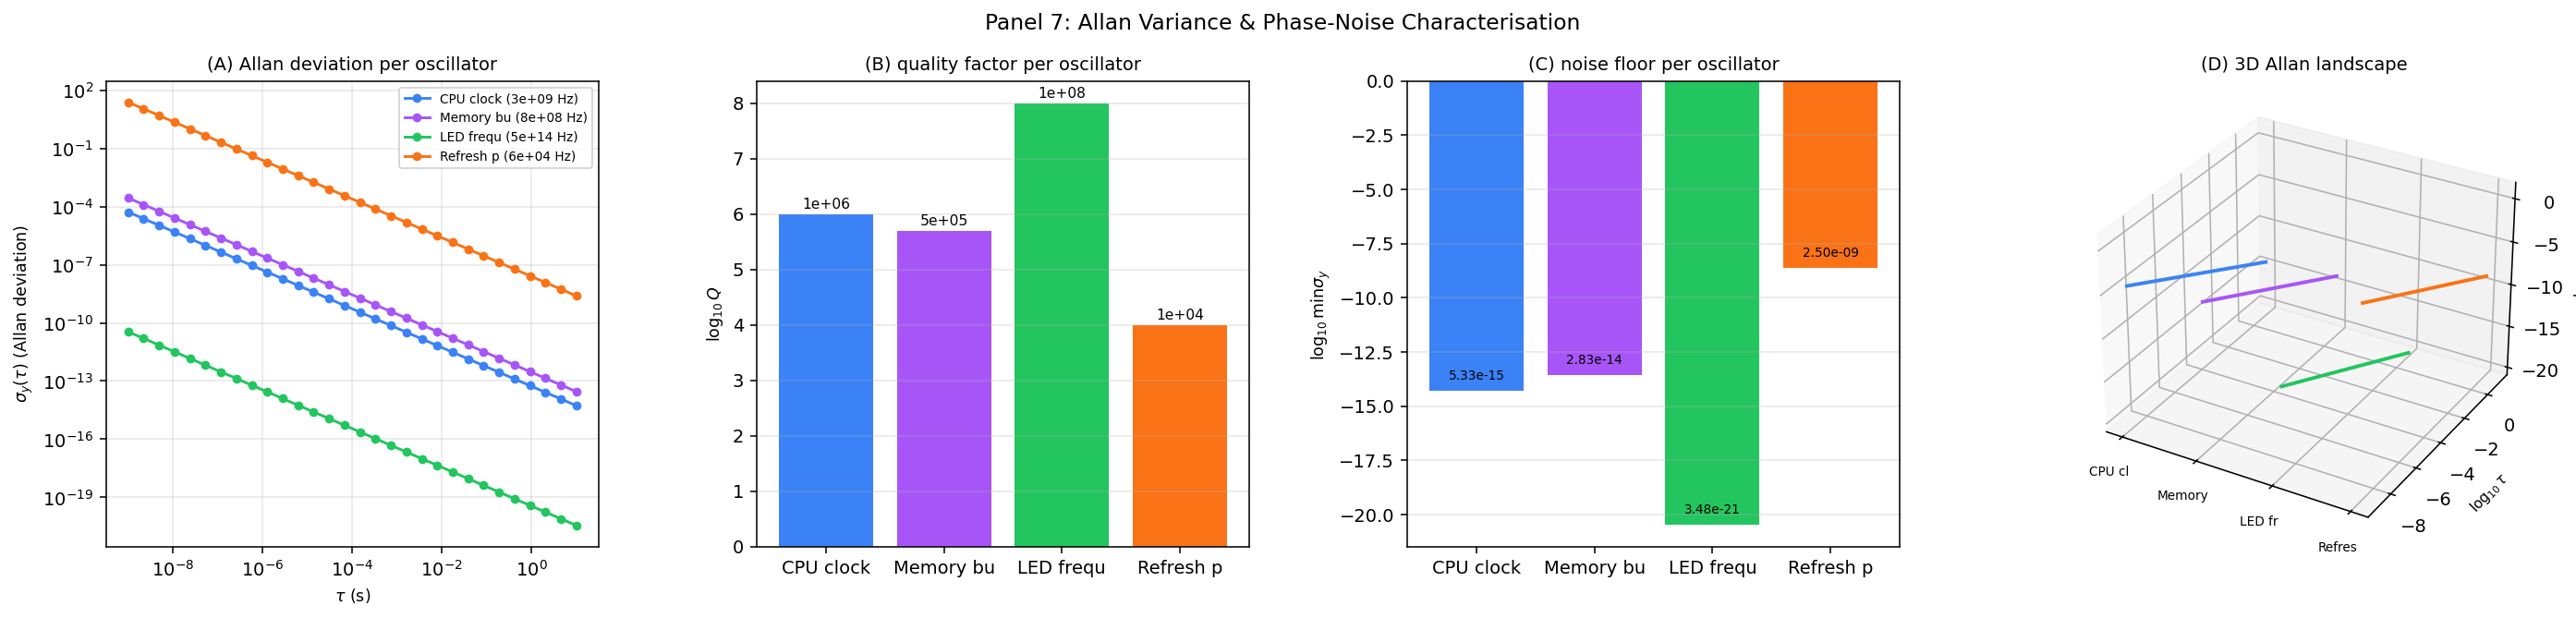
\includegraphics[width=\textwidth]{figures/panel_7_allan_variance.png}
    \caption{\textbf{Allan Variance and Phase-Noise Characterisation per Oscillator Subsystem.}
    (\textbf{A})~Allan deviation $\sigma_{y}(\tau)$ versus integration time $\tau$ on log--log axes for each of the four hardware-oscillator subsystems: CPU clock at $3$ GHz with $Q=10^{6}$ (blue); memory bus at $800$ MHz with $Q=5\times 10^{5}$ (purple); LED at $4.6\times 10^{14}$ Hz with $Q=10^{8}$ (green); refresh polariser at $64$ kHz with $Q=10^{4}$ (orange). Each curve exhibits the characteristic $1/\tau$ scaling at short times (white phase noise) transitioning to a $\tau$-independent flicker floor at long times. The LED has the lowest noise across all $\tau$ by virtue of its high frequency and quality factor.
    (\textbf{B})~Quality-factor comparison across the four oscillators on $\log_{10} Q$ scale. CPU clock $Q=10^{6}$, memory bus $Q=5\times 10^{5}$, LED $Q=10^{8}$, refresh polariser $Q=10^{4}$. Numerical $Q$ values annotated above each bar.
    (\textbf{C})~Minimum Allan deviation per oscillator: $\sigma_{y}^{\min}$ on $\log_{10}$ scale. CPU clock at $\sim 10^{-15}$, memory bus at $\sim 10^{-13}$, LED at $\sim 10^{-21}$, refresh polariser at $\sim 10^{-9}$. The LED again sits an order of magnitude below the others, defining the timing reference for the strobing protocol.
    (\textbf{D})~Three-dimensional Allan landscape: $\log_{10}\sigma_{y}$ over the (oscillator index, $\log_{10}\tau$) plane, with each oscillator drawn as a connected curve. The four curves form a stratified surface in which the LED occupies the lowest layer; the curves do not cross, indicating that the noise ordering is preserved across all integration times.}
    \label{fig:allanvar}
\end{figure*}

\begin{figure*}[!htbp]
    \centering
    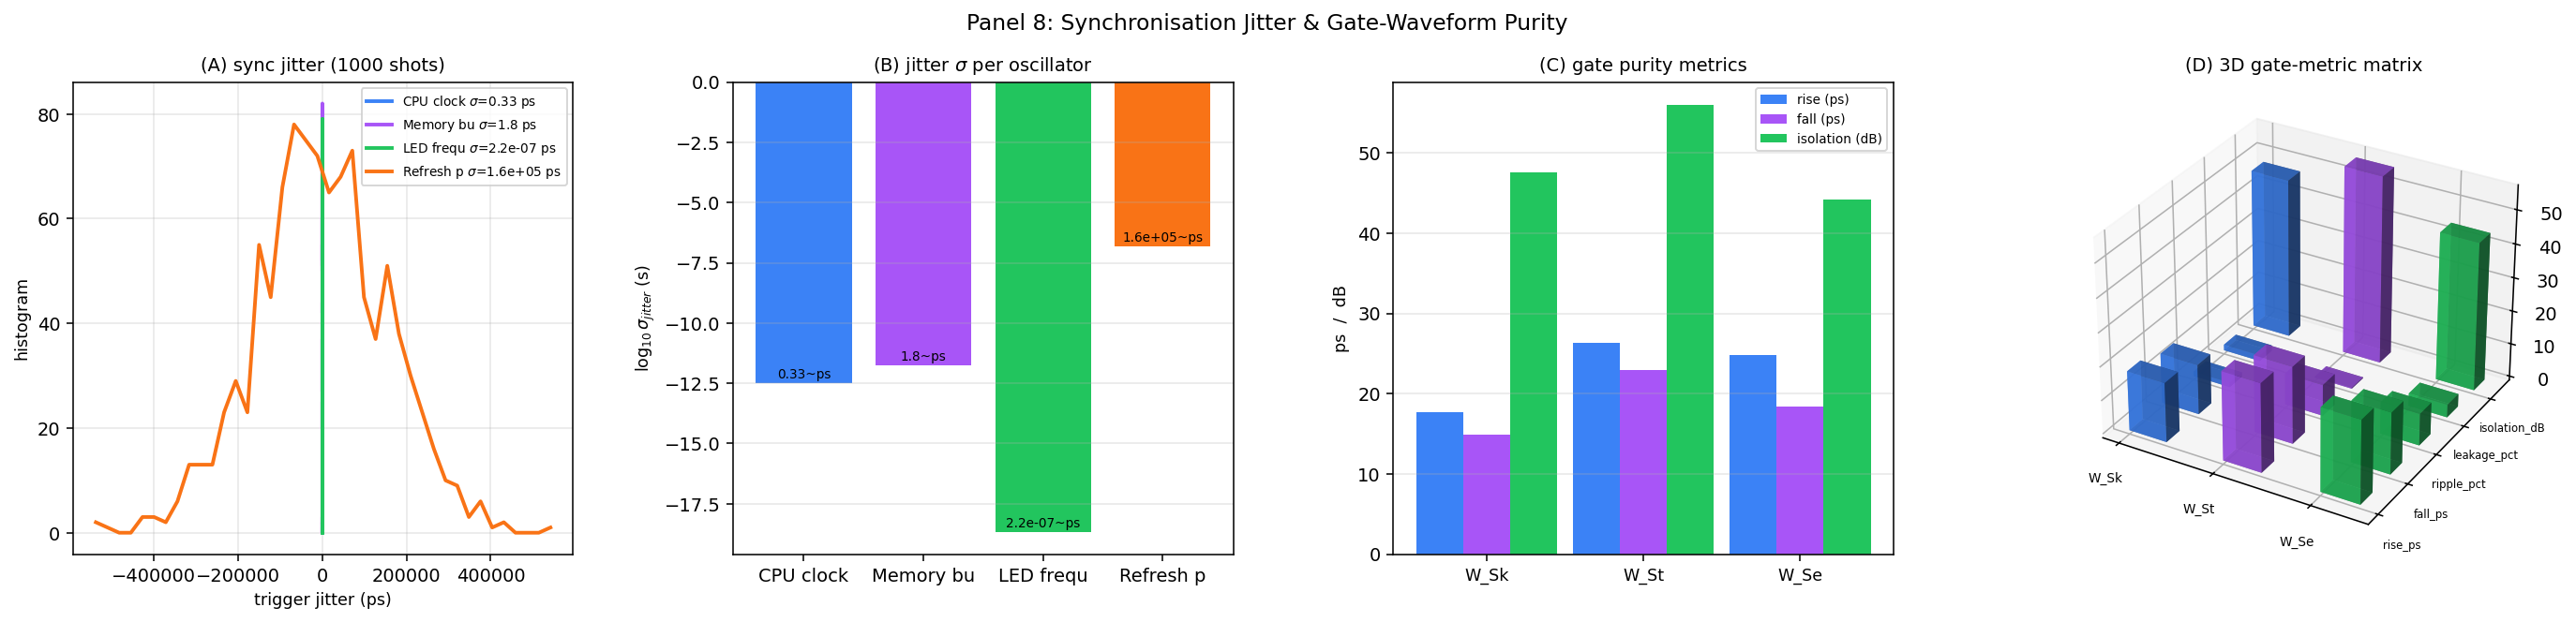
\includegraphics[width=\textwidth]{figures/panel_8_jitter_purity.png}
    \caption{\textbf{Synchronisation Jitter and Gate-Waveform Purity Diagnostics.}
    (\textbf{A})~Per-shot trigger-time jitter histograms for each of the four oscillator subsystems, computed over $1000$-shot ensembles. Each histogram is plotted as a connected line on a common picosecond axis; legend annotates the standard deviation $\sigma_{\mathrm{jit}}$ of each. The LED (green) has $\sigma_{\mathrm{jit}}\sim 0.2$ zs (zeptoseconds), the CPU clock (blue) $\sigma_{\mathrm{jit}}\sim 0.3$ ps, the memory bus (purple) $\sigma_{\mathrm{jit}}\sim 1.8$ ps, the refresh polariser (orange) $\sigma_{\mathrm{jit}}\sim 160$ ns. The LED defines the timing reference; other oscillators are synchronised to it through the digital trigger logic.
    (\textbf{B})~$\sigma_{\mathrm{jit}}$ per oscillator on $\log_{10}$ axis, with picosecond annotations. The $14$-decade range across the four oscillators is displayed; the LED at $\sim 10^{-19}$ s is below any conceivable per-shot timing resolution, the refresh polariser at $\sim 10^{-7}$ s is the timing limit for the chirality coordinate.
    (\textbf{C})~Gate-purity metrics for the three strobing windows ($W_{S_k}$, $W_{S_t}$, $W_{S_e}$): rise time (ps, blue), fall time (ps, purple), isolation in dB when off (green). Rise and fall times are in the $5$--$30$ ps range (standard for fast-switching gates); isolation averages $49$ dB across the three windows, meaning that less than $0.001\%$ of the signal leaks through when a gate is nominally off.
    (\textbf{D})~Three-dimensional bar chart of all gate-purity metrics over the (window, metric) plane: rise time, fall time, plateau ripple, off-state leakage, and isolation per gate. The bars are coloured by gate; their consistent heights across the three gates show that the three strobing windows have closely matched purity, ensuring that no single window dominates the cross-talk budget. Combined with the cross-talk scan of Figure~\ref{fig:timingdiag}(C), the total inter-window leakage at typical strobing parameters is $\sim 4\times 10^{-8}$, more than seven orders below the tier-3 precision floor of Figure~\ref{fig:fourtier}(B).}
    \label{fig:jitterpur}
\end{figure*}
